%\documentstyle[10pt,twoside]{article}
%\documentstyle[twoside]{article}
\documentclass[twoside]{article}
\setlength{\oddsidemargin}{0.25 in}
\setlength{\evensidemargin}{-0.25 in}
\setlength{\topmargin}{-0.6 in}
\setlength{\textwidth}{6.5 in}
\setlength{\textheight}{8.5 in}
\setlength{\headsep}{0.75 in}
\setlength{\parindent}{0 in}
\setlength{\parskip}{0.1 in}

\usepackage{graphicx}
\usepackage{url}

%
% The following commands sets up the lecnum (lecture number)
% counter and make various numbering schemes work relative
% to the lecture number.
%
\newcounter{lecnum}
\renewcommand{\thepage}{\thelecnum-\arabic{page}}
\renewcommand{\thesection}{\thelecnum.\arabic{section}}
\renewcommand{\theequation}{\thelecnum.\arabic{equation}}
\renewcommand{\thefigure}{\thelecnum.\arabic{figure}}
\renewcommand{\thetable}{\thelecnum.\arabic{table}}
\newcommand{\dnl}{\mbox{}\par}

%
% The following macro is used to generate the header.
%
\newcommand{\lecture}[4]{
   \pagestyle{myheadings}
   \thispagestyle{plain}
   \newpage
   \setcounter{lecnum}{#1}
   \setcounter{page}{1}
   \noindent
   \begin{center}
   \framebox{
      \vbox{\vspace{2mm}
    \hbox to 6.28in { {\bf CMPSCI~677~~~Operating Systems
                        \hfill Spring 2018} }
       \vspace{4mm}
       \hbox to 6.28in { {\Large \hfill Lecture #1: #2  \hfill} }
       \vspace{2mm}
       \hbox to 6.28in { {\it Lecturer: #3 \hfill Scribe: #4} }
      \vspace{2mm}}
   }
   \end{center}
   \markboth{Lecture #1: #2}{Lecture #1: #2}
   \vspace*{4mm}
}

%
% Convention for citations is authors' initials followed by the year.
% For example, to cite a paper by Leighton and Maggs you would type
% \cite{LM89}, and to cite a paper by Strassen you would type \cite{S69}.
% (To avoid bibliography problems, for now we redefine the \cite command.)
%
\renewcommand{\cite}[1]{[#1]}

% \input{epsf}

%Use this command for a figure; it puts a figure in wherever you want it.
%usage: \fig{NUMBER}{FIGURE-SIZE}{CAPTION}{FILENAME}
\newcommand{\fig}[4]{
            %\vspace{0.2 in}
            \centerline{\includegraphics[scale=#2]{#4}}
            \begin{center}
            Figure \thelecnum.#1:~#3
            \end{center}
    }

% Use these for theorems, lemmas, proofs, etc.
\newtheorem{theorem}{Theorem}[lecnum]
\newtheorem{lemma}[theorem]{Lemma}
\newtheorem{proposition}[theorem]{Proposition}
\newtheorem{claim}[theorem]{Claim}
\newtheorem{corollary}[theorem]{Corollary}
\newtheorem{definition}[theorem]{Definition}
\newenvironment{proof}{{\bf Proof:}}{\hfill\rule{2mm}{2mm}}

% Some useful equation alignment commands, borrowed from TeX
\makeatletter
\def\eqalign#1{\,\vcenter{\openup\jot\m@th
  \ialign{\strut\hfil$\displaystyle{##}$&$\displaystyle{{}##}$\hfil
      \crcr#1\crcr}}\,}
\def\eqalignno#1{\displ@y \tabskip\@centering
  \halign to\displaywidth{\hfil$\displaystyle{##}$\tabskip\z@skip
    &$\displaystyle{{}##}$\hfil\tabskip\@centering
    &\llap{$##$}\tabskip\z@skip\crcr
    #1\crcr}}
\def\leqalignno#1{\displ@y \tabskip\@centering
  \halign to\displaywidth{\hfil$\displaystyle{##}$\tabskip\z@skip
    &$\displaystyle{{}##}$\hfil\tabskip\@centering
    &\kern-\displaywidth\rlap{$##$}\tabskip\displaywidth\crcr
    #1\crcr}}
\makeatother

% **** IF YOU WANT TO DEFINE ADDITIONAL MACROS FOR YOURSELF, PUT THEM HERE:



% Some general latex examples and examples making use of the
% macros follow.

\begin{document}

%FILL IN THE RIGHT INFO.
%\lecture{**LECTURE-NUMBER**}{**DATE**}{**LECTURER**}{**SCRIBE**}
\lecture{22}{April 8}{Jeremy Gummeson}{\textbf{James Woglom}}

\section{Introduction}

Jeremy Gummeson is a Senior Research Fellow at UMass, and a former research scientist at Hewlett Packard Labs and Disney Research. He works in the UMass Sensors and Laboratory for Advanced System Software labs.

\section{Pervasive Computing}

Pervasive or ubiquitous computing refers to the fact that computers and connected technology is becoming incorporated transparently around us, from places like our own wrist to the buildings we're in. Smartphones are nearly ubiquitous, and contain significant numbers of sensors. Computing is also increasingly becoming a part of physical environments, e.g. with smart homes and IoT devices.

Four major subsections of 

\subsection{Rise of Pervasive Computing}

\begin{itemize}
  \item Miniturization (Moore's Law); for example, Microelectromechanical systems (MEMS) are microscopic devices at a very small scale.
  \item Sensors have become more powerful and efficient. For example, look at how powerful smartphones have become.
\end{itemize}

\subsection{Applications}

\subsubsection{Smart Health}
Early wearable devices can track aspects relating to fitness, such as heart rate and serve as a step counter, as well as perform sleep tracking. Newer devices, some commercially available and some still in research, include smart clothing (devices embedded into clothing which can do on-body detection of, e.g., sweat detection) and smart glasses (which can track your eye pupil movements to detect fatigue).

\subsubsection{Smart Buildings}
Smart buildings includes connected thermostats (allowing you to adjust the temperature and view it remotely), smart plugs (being able to turn on and off devices remotely), smart appliances (e.g., a fridge or washing machine), and smart locks. 

Smart buildings also encompasses devices like the Amazon Echo and Google Home, which serve as voice assistant devices, and also can be configured in mesh layouts where no matter where you are located in your home, a device can still hear you. This can help create a cohesive smart home ecosystem; for example, the Nest Thermostat can be controlled via phone or voice using a smart assistant.

\subsubsection{Smart Transportation}
Smart transportation involves both infrastructure and device improvements. With smart roadways, roads can have dynamically-adjusting lanes, speed limits, and reactive lights (which conserves energy). 

With connected cars, an ongoing research topic involves fleet management, wherein cars would create a local area network using a Bluetooth-like protocol to be able to inform each other about their positions and prevent crashes.

\subsection{Infrastructure Design}
A typical example of the way in which smart devices work involves communication from the personal device to a wearer's smartphone, which is then connected to the internet and can communicate with servers in the cloud to sync data. The device to phone communication likely occurs via Bluetooth LE or a similar low-power technology. For devices that are more stationary, an environmental sensor can connect directly to the internet via a home network (e.g., with your home WiFi network), and then communicate with the cloud.

A dashboard interface can then likely serve as the way in which a user views the output of these devices, and that dashboard interface could either be a website which reads database data that was synced from the devices or reads from the devices directly over the network.

\subsection{Sensor Platforms}


\subsubsection{CPU}
Low-powered sensor nodes can be thought of as a resource-constrained distributed system. They typically use a small CPU (8-bit addressable bus, 4KB of RAM), a low powered radio transmitter (with rates of between 10 and 200 Kbit/sec), whichever sensors are needed for the application, a small amount of flash storage to store the OS and application components, and either a battery and/or a mechanism which allows the sensor to be self-powered (like a solar panel, for instance).

For example: an Atmel AVR (8-bit data path, 4KB RAM, 128KB flash-on-chip, around 8 mA of power consumption), a TI MSP430 (16-bit data path, 10KB RAM, 48KB flash), or a Raspberry Pi (ARM v6/v7, much closer to a smartphone in terms of processing ability).

\subsubsection{Low-Power Radios}
The ISM Band (Industrial, Scientific and Medical Radio Band) is often used for low-power communication between nodes, especially the 900MHz and 2.4GHz ranges. These band ranges are available for general use by communication equipment without registration via the FCC or other bodies. 

Varying levels of modulation and different protocols are used, such as Zigbee which modulates the phase of radio waves and Bluetooth which modules the frequency. These methods are used for short-range, less than 100m communication.

There are some emerging methods and protocols currently under testing and development. The Chipcon CC2420 is an extremely low-power radio, requiring only 9-17mA of power to transmit and 19mA to receive. As is generally true across radio communication methods, listening for signals requires slightly more energy than transmitting.

\subsubsection{Battery Power}
The Mica2 Mote, a common mid-2000s sensor node, required 2 AA batteries and used 25mA of power. This provided around 100hrs of lifetime.

Some alternatives to provide for longer battery life include:
\begin{itemize}
  \item Bigger batteries (duh.)
  \item Energy harvesting, which are methods which allow for the system itself to generate the power that it needs to operate. This might include motion, wind, or solar. In some cases, the thing being observed via the sensor can actually provide some energy which can then be used to power the sensor. Self-harvesting allows nodes to harvest energy from the environment to power themselves. This includes solar panels, vibration, thermal, airflow, and wireless energy transfer.
  \item Duty cycling, which involves waking up periodically and then sleeping a fixed amount. Methods can be used which allow for duty cycling without missing messages, if nodes' wakeup times are synchronized.
  \item Use of higher-order sensors, which require less energy. When a higher-order sensor is activated, then the lower-level sensor which requires more energy is activated. That way the lower-level sensor is only activated when it is predicated that the thing being observed is actually present or some change has occurred.
\end{itemize}

\subsection{Types of Sensors}
An incomplete list:
\begin{enumerate}
  \item Temperature
  \item Humidity
  \item Magnetometer
  \item Vibration
  \item Acoustic
  \item Light
  \item Motion/IR
  \item Imaging
  \item Accelerometer
  \item Location/GPS
\end{enumerate}

Most of these sensors are now included in modern smartphones.


\subsection{Typical Design Issues}

For a single node:
\begin{itemize}
  \item Battery power
  \item How to harvest energy to maximize lifetime  
\end{itemize}

For a network of sensors:
\begin{itemize}
  \item Data aggregation
  \item Duty cycling
  \item Localization/synchronization
  \item Routing
\end{itemize}

Outside of the network (server-side processing)
\begin{itemize}
  \item Big data analytics
  \item Deriving insights from the data
  \item Sending alerts
  \item Providing active control of the nodes by an operator
\end{itemize}

\section{Green Computing}
How do you design energy efficient hardware/software/systems? Nowadays, IT is used to make infrastructure efficient.

Greening of Computing is an attempt to design energy-efficient hardware/software/systems, while computing for greening refers to the use of computers to make physical infrastructure more efficient.

\subsection{Historical Overview}
Energy efficient mobile devices are a long-standing problem. The recent growth of datacenters has resulted in a large focus on energy efficiency in server farms, because it lowers the operating cost.

\subsection{Datacenter Power Consumption}
Computers often require 20\% of the power usage in office buildings, 50-80\% of the power usage at a large college and, globally, $>$3\% of our carbon footprint.

Datacenters encompass servers, network gear, and storage infrastructure. Google's Dallas DC requires 100MW of power to operate, and the server cost per KwH is \$50/month.

\subsection{Green Datacenters}
Green datacenters reduce the cost of running servers and cooling, and use green infrastructure practices. They use more energy-efficient servers and manage their servers better collectively. 

In order to reduce cooling costs, some innovative approaches for HVAC/air conditioning systems have been employed by thermal engineers. Naturally cooled datacenters are one option: build datacenters in Iceland!

\section{Personal Research Projects}

\subsection{Battery-Free IoT (Disney Research)}
Because RFID tags don't require battery power to operate (a capacitor is charged by the 900MHz signal emitted by a receiver), research has been done on ways to operate IoT systems using RFID. They have a read rate of around 50 samples/sec.

Challenges with ubiquitous RFID:
\begin{itemize}
  \item Routing power and communications to readers is difficult
  \item Antennas need to be large to achieve good coverage
  \item Antennas need line of sight to tags
\end{itemize}

Idea: reuse home infrastructure, by incorporating a RFID reader in a lightbulb.

\subsubsection{Setup Overview}
\begin{itemize}
  \item Install light bulbs and associate with Wi-Fi AP
  \item Install tags and register with backend server
  \item Interpret data, which can be used to actuate lighting and UI
\end{itemize}

\subsubsection{Hardware Design}
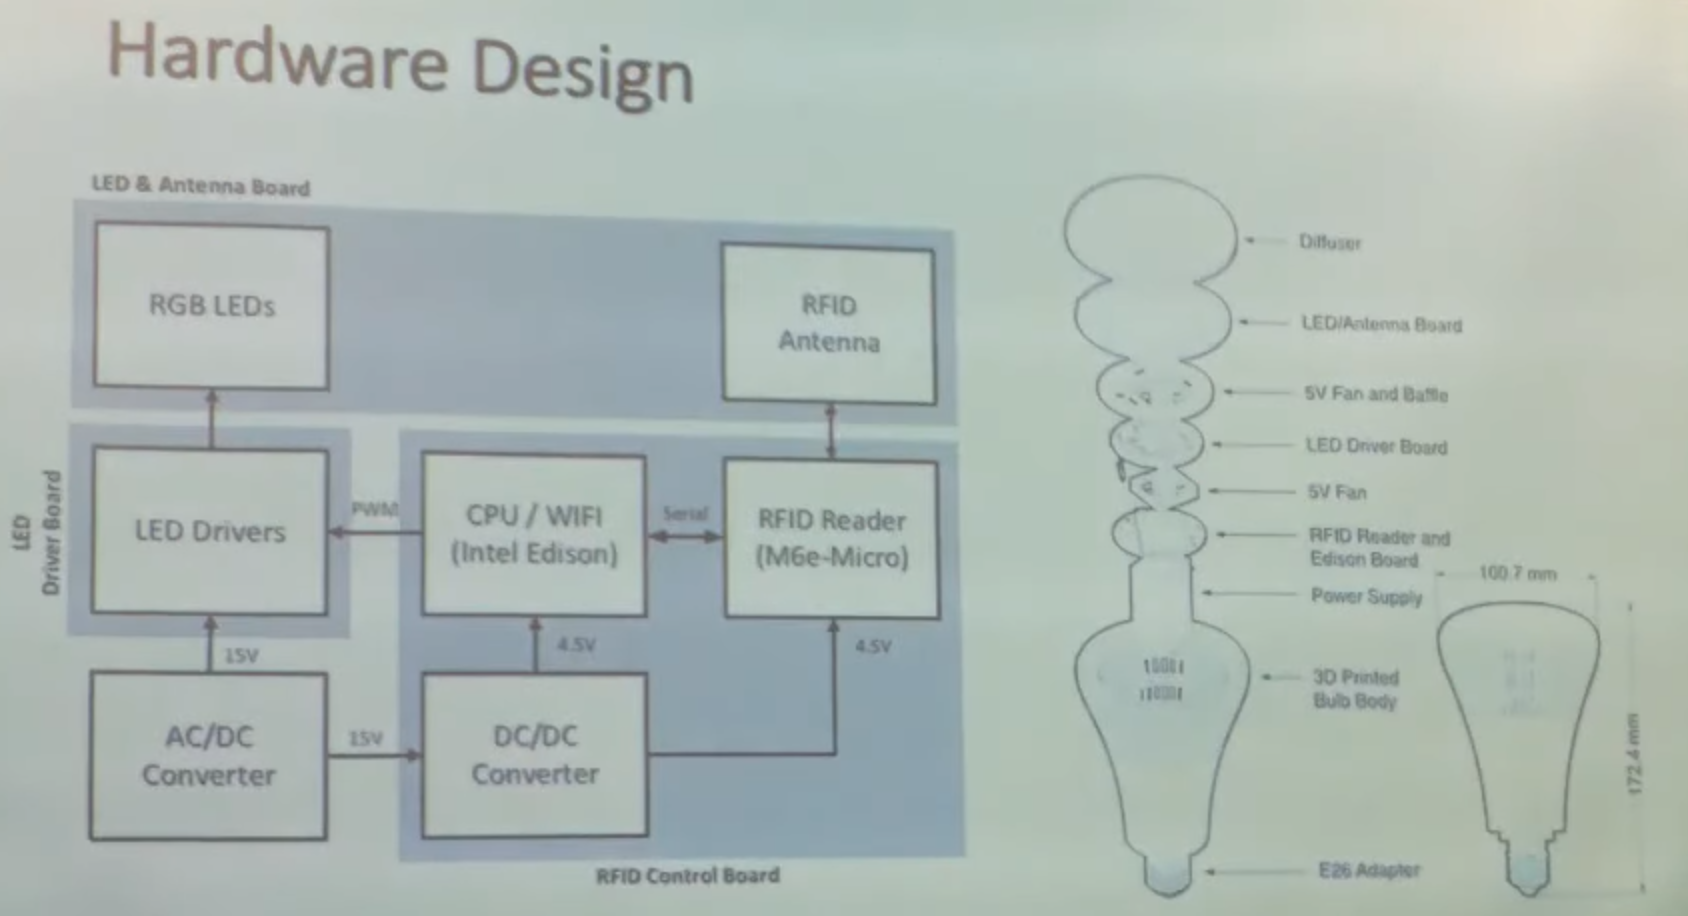
\includegraphics[scale=0.6]{hwdesign.png}

\subsubsection{Interactive RFID Tags}
\begin{itemize}
  \item Location
  \item Thermostat
  \item Touch
  \item Temperature
  \item Contact switch
\end{itemize}

\subsubsection{Classes of Applications}
To showcase the applications enabled by networks of RFID lightbulbs, three application categories were explored that leverage the scale of coverage and immediate feedback that RFID lightbulbs provide.
\begin{itemize}
  \item Navigation
  \item Infrastructure Monitoring
  \item Prepackaged Content
\end{itemize}

\section{Summary}
"Greening" of computing for IoT and Health:
\begin{itemize}\item Designing energy efficient hardware and software.
  
\end{itemize}


Computing for greening:
\begin{itemize}
  \item Use of IT for monitoring, analytics, and control
  \item Use of intelligent software for power management
  \item Forecasting for reasonable energy harvesting
\end{itemize}
Emerging IoT technologies: 
\begin{itemize}
  \item Battery-free sensing with RFID sensors
  \item 5G networks
\end{itemize}
\end{document}
